\LevelOneTitle{管道内流动}

\LevelTwoTitle{圆管湍流特性}

\begin{figure}[H]
	\centering
	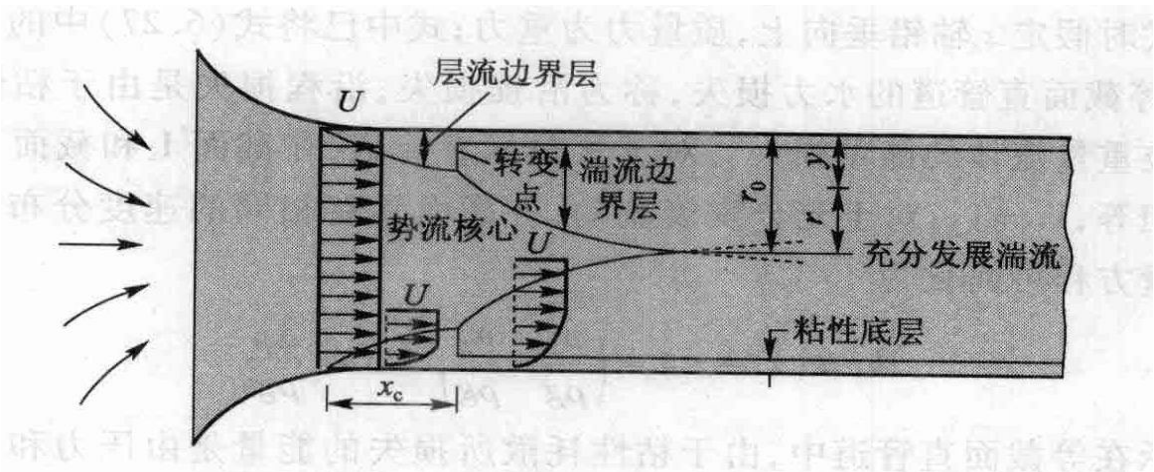
\includegraphics[scale=0.3]{figures/圆管湍流.png}
	\caption{圆管湍流示意}
\end{figure}

势流核心区短,粘性区域厚度增加快,达到充分发展需要的长度长,充分发展段:速度分布更均匀,沿流动方向速度分布不变,过流断面上切应力分布相同,速度分布相同,压降与$x$成线性关系(单位压降相同),压力(有时也有重力)和粘性力平衡。

$Re$增大,起始段长度增加,充分发展段速度分布更均匀。

\LevelTwoTitle{实际总流伯努利方程}

\begin{equation}
	\dfrac{\alpha_1 \overline{V}_1^2}{2g} + z_1 + \dfrac{p_1}{\rho g} = \dfrac{\alpha_2 \overline{V}_2^2}{2g} + z_2 + \dfrac{p_2}{\rho g} + h_f + h_{\text{轴}}
\end{equation}

式中$\alpha$的取值需要根据流态确定,$Re > Re_{cr} = 2300$,湍流,$\alpha = 1$;$Re < Re_{cr} = 2300$,层流,$\alpha = 2$(考试一般都是湍流,但仍需要先判断再取值)。

物理意义可以参照总流伯努利方程来写,注意加上水里损失和轴功影响。

适用条件:

\begin{enumerate}
	\item 不可压缩流动;
	\item 定常;
	\item 质量力有势且只有重力;
\end{enumerate}

\LevelTwoTitle{水力损失和轴功}

\begin{definition}[水力损失$h_f$]
	单位重量流体由1点流到2点克服粘性力损失的能量(机械能),分为沿程阻力损失$h_l$和局部阻力损失$h_m$,即$h_f = \sum h_l + \sum h_m$。
\end{definition}

\LevelThreeTitle{圆管沿程阻力损失}

沿程阻力损失是流体在均直管道内克服摩擦阻力做功,损失的能量可能来自压力能(水平管道)和重力势能(非水平管道),数学表达为

\begin{equation}
	h_l = f \dfrac{l}{D} \dfrac{\overline{V}^2}{2g} \label{eq9.2}
\end{equation}

其中,

\begin{enumerate}
	\item 圆管层流,$f = \dfrac{64}{Re}$;
	\item 圆管湍流,$f = 0.11\qty(\dfrac{68}{Re} + \dfrac{\Delta}{D})^{0.25}$(水力粗糙);$f = \dfrac{0.3164}{Re^{0.25}}$(*水力光滑)。
\end{enumerate}

\LevelThreeTitle{非圆管沿程阻力损失}

只需令式\ref{eq9.2}中$f = \dfrac{C}{Re_h}$和$D \to D_h = \dfrac{4A}{P}$即可。

其中,$C$与截面形状尺寸有关,$D_h$称为当量直径(水力直径),$A$为过流断面面积,$P$为湿周,是粘性应力作用的所有周长。

\begin{tip}
	此处可能考选择题,考查水力直径、湿周的定义等,计算大题应该还是圆管。
\end{tip}

\LevelThreeTitle{局部阻力损失(2021·简答)}

局部阻力损失是经过各种管道构件和管道连接件产生的损失,具体原因是发生了速度场突变、流体元碰撞,甚至是流体分离形成旋涡,数学表达为

\begin{equation}
	h_m = K\dfrac{\overline{V}^2}{2g}
\end{equation}

其中,$K$取决于管件几何形状、尺寸和流动的$Re$,当$Re$很大时,$K$与$Re$无关。题目中一般会给$K$的值,但仍建议记忆出入口处的$K$值。

\begin{enumerate}
	\item $A_2 \gg A_1$,$K = 1$;
	\item $A_1 \gg A_2$,$K = 0.5$。
\end{enumerate}

大口变小口损失小,小口变大口损失大。

\LevelThreeTitle{轴功}

\begin{enumerate}
	\item $h_{\text{轴}} < 0$,表明机械向流体作功,例如水泵;
	\item $h_{\text{轴}} > 0$,表明流体向机械作功,例如水轮机;
	\item 功率$\dot{W} = \rho g Q \abs{h_{\text{轴}}}$。
\end{enumerate}

\LevelTwoTitle{*穆迪图的四个区域}

\begin{enumerate}
	\item 层流区,$f = \dfrac{64}{Re}$;
	\item 水力光滑区,$f = f(Re)$;
	\item 过渡粗糙区,$f = f(Re, \dfrac{\Delta}{D})$;
	\item 完全粗糙区,$f = f(\dfrac{\Delta}{D})$。
\end{enumerate}

\LevelTwoTitle{串、并联管道}

\begin{enumerate}
	\item 串联
	\begin{align*}
		&Q_1 = Q_2 = Q_3 = \cdots\\
		&h_f = \sum h_{f_i}
	\end{align*}
    \item 并联
    \begin{align*}
    	&Q = \sum Q_i\\
    	&h_{f_1} = h_{f_2} = h_{f_3} = \cdots
    \end{align*}
\end{enumerate}

\LevelTwoTitle{例题练习}

\begin{example}
	如图,运动粘度$\nu = 5.16 \times 10^{-6}$ m$^2$/s,密度$\rho = 861$ kg/m$^3$的燃油通过长1830 m,内径为$d = 400$ mm的铆接钢管($\varepsilon = 2$ mm)输送到油池C。流量为0.2 m$^3$/s时,A点表压为13.8 kPa。试求泵AB的输出功率和B点的压强,忽略局部阻力损失。
	
	\begin{figure}[H]
		\centering
		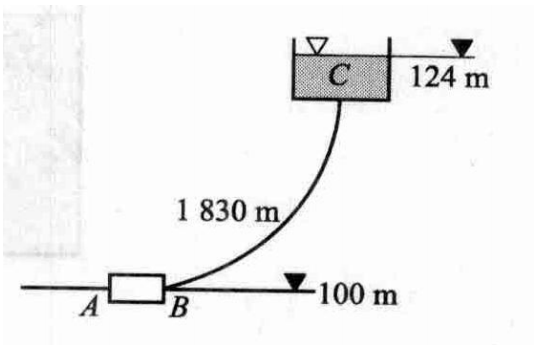
\includegraphics[scale=0.4]{figures/C9-fig1.png}
		\caption{例图}
	\end{figure}

    \begin{enumerate}
    	\item 雷诺数
    	\begin{equation*}
    		Re = \dfrac{Vd}{\nu} = \dfrac{4Q}{\pi \nu d} = \dfrac{4 \times 0.2}{\pi \times 5.16 \times 10^{-6} \times 0.4} = 123376 \gg 2300
    	\end{equation*}
        故该流动为湍流,动能修正系数$\alpha = 1$。
        \item 沿程阻力损失
        \begin{align*}
        	&f = 0.11 \qty(\dfrac{68}{Re} + \dfrac{\varepsilon}{d})^{0.25} = 0.11 \times \qty(\dfrac{68}{123376} + \dfrac{2}{400})^{0.25} = 0.03\\
        	&h_l = f \dfrac{l}{d} \dfrac{V^2}{2g} = f \dfrac{l}{d} \dfrac{8Q^2}{\pi^2 d^4 g} = 0.03 \times \dfrac{1830}{0.4} \times \dfrac{8 \times 0.2^2}{\pi^2 \times 0.4^4 \times 9.8} \mathrm{~m} = 17.74 \mathrm{~m}
        \end{align*}
        \item 取A,C两处列伯努利方程
        \begin{equation*}
        	\dfrac{V^2}{2g} + z_A + \dfrac{p_A}{\rho g} = \dfrac{V^2}{2g} + z_C + 0 + h_l + h_{\text{轴}}
        \end{equation*}
        解得
        \begin{equation*}
        	h_{\text{轴}} = -40.10 \mathrm{~m} < 0
        \end{equation*}
        表明流体机械向流体输出功。
        \item 泵AB输出功率
        \begin{equation*}
        	\dot{W} = \rho g Q \abs{h_{\text{轴}}} = 861 \times 9.8 \times 0.2 \times 40.10 \times 10^{-3} \mathrm{~kW} = 67.67 \mathrm{~kW}
        \end{equation*}
        \item 对A,B处,由伯努利方程
        \begin{equation*}
        	\dfrac{p_A}{\rho g} = \dfrac{p_B}{\rho g} + h_{\text{轴}}
        \end{equation*}
        解得
        \begin{equation*}
        	p_B = 352.2 \mathrm{~kPa}
        \end{equation*}
    \end{enumerate}
\end{example}

\begin{tip}
	考试中本章必涉及一道计算,并且会考虑局部阻力损失(本题没有考虑),可以参考课后习题9.25掌握局部阻力损失的计算。
\end{tip}
